\documentclass[a4paper,10pt]{article}

\usepackage{multicol}
\usepackage{caption}
\usepackage[utf8]{inputenc}
\usepackage{hyperref}
\usepackage[left=2.5cm,right=2.5cm,bottom=2cm,top=1cm]{geometry}
\usepackage{authblk}
\usepackage{graphicx}
\usepackage{subfigure}
\usepackage{amsmath}


\usepackage{tikz}
\usetikzlibrary{calc}

\tikzset{egrid/.style={draw,help lines}}
\tikzset{mgrid/.style={draw,help lines,dashed}}
\tikzset{epoint/.style={draw,circle,red,inner sep=2pt,fill}}
\tikzset{mpoint/.style={draw,circle,blue,inner sep=2pt,fill}}

\graphicspath{{./Slike/}}

\title{\textbf{MODELLING LIGHT PROPAGATION THROUGH NON-UNIFORM ANISOTROPIC MATERIALS}}
\author[1]{\textbf{Miha \v Can\v cula\thanks{miha.cancula@student.fmf.uni-lj.si}}}
\author[1,2]{\textbf{Miha Ravnik}}
\author[1,2,3]{\textbf{Slobodan \v Zumer}}
\affil[1]{\textbf{Faculty of Mathematics and Physics, University of Ljubljana, Slovenia}}
\affil[2]{\textbf{Centre of excellence NAMASTE, Ljubljana, Slovenia}}
\affil[3]{\textbf{Jo\v zef Stefan Institute, Ljubljana, Slovenia}}
\date{}

\renewcommand\Authands{ and }


\newcommand{\odvod}[2]{\frac{\partial #1}{\partial #2}}
\renewcommand{\vec}{\mathbf}
\newcommand{\eps}{\varepsilon}
\newcommand{\E}{\vec E}
\newcommand{\B}{\vec B}
\newcommand{\angl}[1]{(\textit{angl. #1})}

\renewcommand\refname{REFERENCES}
  
\begin{document}

\vspace{-6cm}

\maketitle

\thispagestyle{empty}

\vspace{-1cm}

\section*{ABSTRACT}

{\Large 
Liquid crystals are central to modern optics and photonics due to their birefringence and the possibility of external control. 
We present a method for modelling the propagation of light through non-uniform and optically anisotropic materials. 
It is based on the finite-difference time-domain (\textsc{FDTD}) method which evolves electromagnetic fields according to Maxwell's equations\cite{taflove}. 
Unlike other methods for modelling the flow of light, such as Jones' matrices or the Berreman method, it can describe arbitrarily complex structures which occur in liquid crystals\cite{berreman,hwang-rey}. 
}

{\Large
With the newly-implemented method, we modelled reflection and differaction at an interface between materials with different refractive indexes. 
We calculated the transmittance of a liquid crystal layer between crossed polarizers, which agrees with observations and theoretical predictions. 
The method correctly predicted the position of photonic band gap in 1D photonic crystals, as seen on Figure. 
Additionally, more optically complex liquid crystalline structures can be considered.
}

\begin{figure}[h!]
\centering
\begin{minipage}{.45\textwidth}
  \centering
  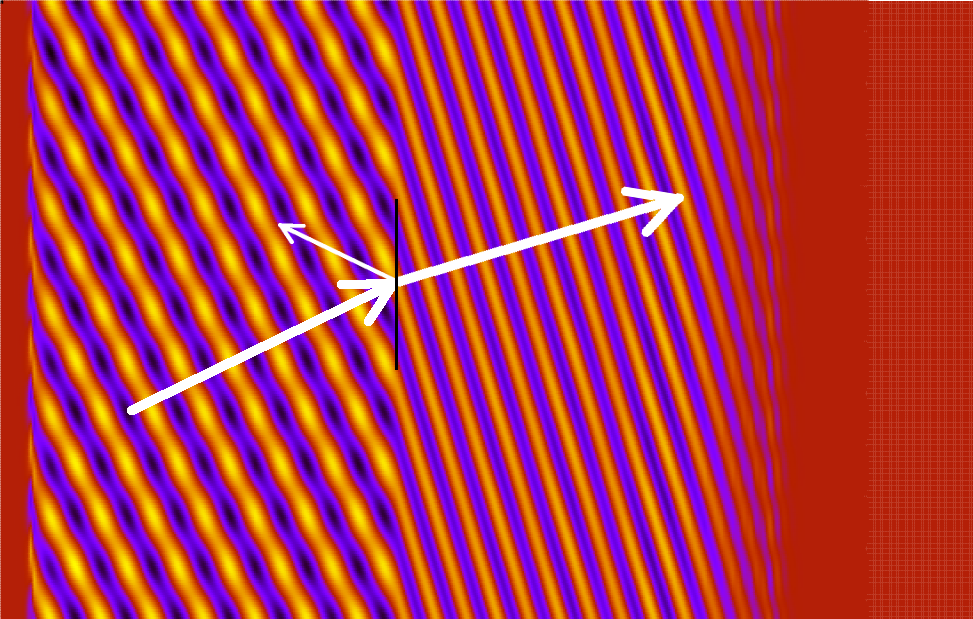
\includegraphics[width=\textwidth]{refraction_t}
  \captionof{figure}{Reflection and refraction at an interface near Brewster's angle. Colors show local electric field, while arrows show the direction of propagation of light.}
  \label{fig:test1}
\end{minipage}%
\hspace{.05\textwidth}
\begin{minipage}{.45\textwidth}
  \centering
  \resizebox{\textwidth}{!}{\input{g_test_periodic_en}}
  \captionof{figure}{Transmittance of a 1D photonic crystal depending on dielectric constants and the frequency of light}
  \label{fig:test2}
\end{minipage}
\end{figure}

\bibliographystyle{zumer}
\bibliography{magisterij}

\end{document}
